\section{Estimating latent dimensionality and non positive semi-definiteness}
\label{sec:dimest}

\subsection{The problem of estimating latent dimensionality}
\label{sec:ch6:dimest:dimselect}
Across all of the embedding techniques we have discussed thus far, we typically have ignored a relatively substantial problem. In all of these algorithms, a hyperparameter for the embedding technique has, in general, been the latent dimensionality $d$. 

The latent dimensionality is associated with the latent dimensionality of an underlying random network, $\mathbf A$. It is important to clarify that this random network has no real interpretation; it only exists for conceptual (being able to think about what is going on) and theoretical (being able to prove that the embedding approach is reasonable in some concrete context) sake. Without knowing a suitable latent dimensionality $d$, this theoretical and intuitive insight starts to break down. For this reason, it is fairly imperative that we are able to in practice make reasonable guesses about $d$; using the notation we have become accustomed to by this point, we need to be able to estimate it with $\hat d$. 

Let's get a working example together:

\begin{lstlisting}[style=python]
from graspologic.simulations import sbm
import numpy as np

# block matrix
n = 100
B = np.array([[0.6, 0.2], [0.2, 0.4]])
# network sample
A, z = sbm([n // 2, n // 2], B, return_labels=True)
\end{lstlisting}

\subsection{The scree plot}

Throughout any investigation into spectral embeddings, one of the critical summary statistics to look at with respect to your embedding matrix (the matrix being embedded) is its scree plot. 

The \textit{scree plot} is a plot of the singular values of the embedding matrix (the diagonal entries of the singular value matrix $\Sigma$) in sequential (descending) order by their indices: the first (biggest) singular value is in the beginning, and the last (smallest) singular value is at the end. You can get the singular values like this:

\begin{lstlisting}[style=python]
from scipy.linalg import svdvals

# use scipy to obtain the singular values
s = svdvals(A)
\end{lstlisting}

And you can look at the scree plot like this:

\begin{lstlisting}[style=python]
from pandas import DataFrame
import seaborn as sns
import matplotlib.pyplot as plt


def plot_scree(svs, title="", ax=None):
    """
    A utility to plot the scree plot for a list of singular values
    svs.
    """
    if ax is None:
        fig, ax = plt.subplots(1,1, figsize=(10, 4))
    sv_dat = DataFrame({"Singular Value": svs, "Dimension": range(1, len(svs) + 1)})
    sns.scatterplot(data=sv_dat, x="Dimension", y="Singular Value", ax=ax)
    sns.lineplot(data=sv_dat, x="Dimension", y="Singular Value", ax=ax)
    ax.set_xlim([0.5, len(s)])
    ax.set_title(title)

plot_scree(s, title="Scree plot of $L$")
\end{lstlisting}

The scree plot is shown in Figure \ref{fig:ch6:scree}(A). Essentially, the intuition is this: the singular values correspond to the relative amount of ``information'' for each singular vector (left or right) in describing the matrix that you are embedding. Since the singular values are decreasing ($\sigma_1 \geq \sigma_2 \geq ... \geq \sigma_n \geq 0$, as we discussed above) each sequential singular value is less and less important for describing the network that you have embedded. In Figure \ref{fig:ch6:scree}(B), we isolate out the first ten dimensions from this plot.

\begin{figure}[h]
    \centering
    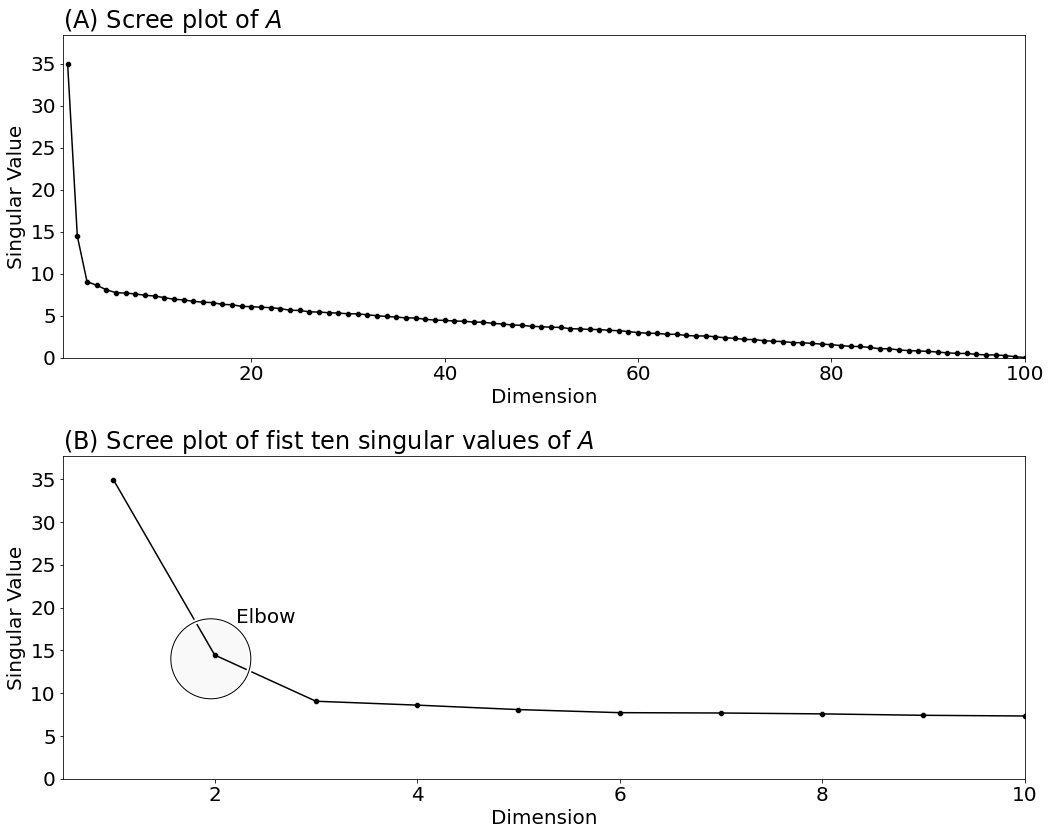
\includegraphics[width=\linewidth]{representations/ch6/Images/scree.png}
    \caption[Scree plot of an adjacency spectral embedding]{\textbf{(A)} the scree plot of singular values of $A$, and \textbf{(B)} the scree plot of the first ten singular values of $A$, with the elbow annotated.}
    \label{fig:ch6:scree}
\end{figure}

You'll notice that there's a marked area called the ``elbow''. This is an area where singular values stop changing in magnitude as much when they get smaller: before the elbow, the singular values decline rapidly, and after the elbow, the singular values ``level off''. It is called an elbow because the plot kind of looks like an arm, viewed from the side.

The location of this elbow gives you a rough indication for how many ``true'' dimensions your latent representation has. The singular values after the elbow are quite close to each other and have singular vectors which are largely noise, and don't tell you very much about your data. It looks from the scree plot that you should be embedding down to two dimensions, as the smaller dimensions tend to be more "noisy" than the first few. The first few will tend to do a good job of describing the overall structure of the matrix that you have embedded, whereas successive dimensions tend to not be as useful. Notice that our example $SBM_n(\vec z, B)$ random network has a true latent position matrix with two latent dimensions, by using the results we obtained in Section \ref{sec:ch5:psd_block:lpm_fromsbm}. This coincides with the location of the elbow on the scree plot for the network sample $A$, so we were able to effectively estimate the true latent dimensionality $d$ using only the data sample $A$. 

\paragraph*{The balancing act of elbow selection}

Particularly when networks have fewer nodes, or when your adjacency matrix has very few non-zero entries, this tends to get rather messy. There may be multiple elbows in your scree plot, and it may be unclear where you should ``draw the line'' and cut off extraneous singular values. By removing too many dimensions, you may end up cutting off dimensions that contain latent structure in your estimated latent positions that you could use downstream to learn about your network. By removing too few dimensions, you may be left with estimated latent positions that have too many latent dimensions, and learning about your network later might be overly complicated. In this sense, there is a balancing act to choosing an estimated latent dimensionality.

\subsection{Automatic elbow selection}

Another drawback to the visual method of estimating latent dimensionality is that a lot of the time, the elbow location is fairly subjective. Real data will rarely have a prominent like the simulated network you see above. The advantage is that it still generally works pretty well; embedding into a few more dimensions than you need isn't too bad, since you'll only have a few noise dimensions and there still may be *some* signal there.

\texttt{graspologic} automates the process of finding an elbow using a popular method developed in 2000 by Dr. Thomas Minka at MIT (called \texttt{minka}, from \cite{Minka2000}). We won't get into the specifics of how it works here, but it generally does a fairly good job at automatic elbow selection. When you use any embedding methods and do not specify a number of embedding dimensions (via the \texttt{n\_components} argument that we used throughout this section), the elbow selection is done automatically:

\begin{lstlisting}[style=python]
from graspologic.embed import AdjacencySpectralEmbed as ase

# use automatic elbow selection
Xhat_auto = ase().fit_transform(A)
\end{lstlisting}

Looking at the number of columns of \texttt{Xhat\_auto.shape[1]} gives you the dimensionality estimated by graspologic. 


\subsection{What happens for non positive semi-definite probability matrices?}
\label{sec:ch6:dimest:grdpg}

\paragraph*{Why did we ignore non positive semi-definite probability matrices?}

Throughout this book, we have taken an overarching intuitive leap: we have conceptualized the underlying random networks to have positive semi-definite probability matrices. This has some extremely convenient implications for us. 

First, we were able to bridge latent position matrices with $DCSBM_n(\vec z, \vec \theta, B)$ and $SBM_n(\vec z, B)$ random networks with positive semi-definite block matrices exactly and succinctly, taking the probability matrices to be:
\begin{align*}
    P_{sbm} &= C B C^\top \\
    P_{dcsbm} &= \Theta C B C\Theta^\top
\end{align*}
where since $B$ was positive semi-definite, it had an exact square-root matrix (which was real) that we could calculate. This allowed you to obtain exact (real) representations of latent positions:
\begin{align*}
    X_{sbm} &= C\sqrt{B} \\
    X_{dcsbm} &= \Theta C \sqrt{B}
\end{align*}
Where we would always be able to compute $\sqrt{B}$ in an exact form (using the Cholesky decomposition, as we did in Section \ref{sec:ch5:psd_block}). 

Second, in order to understand the results in this Chapter, the assumptions that we needed (linear algebra wise) are comparatively easy to wrap your head around; positive semi-definiteness gave us immediate conclusions about the eigendecomposition and the singular value decomposition in Remarks \ref{box:ch6:evd_sum} and \ref{box:ch6:svd_results} respectively. You can find understandable proofs of many of the results that these remarks summarized that are (comparatively) easy to read across numerous linear algebra books \cite{Axler, Trefethen1997} or other online resources. These remarks led to immediate equality of calculations of $P$ (or the population Laplacian $\mathcal L$) using the eigendecomposition and the singular value decomposition, without needing to stray too far from background that would be gained from an introductory linear algebra course, which we believe is fairly important to being able to nail the concepts down in your head appropriately. 

Finally, positive semi-definite structure tends to arise readily in real data. It is a context that you will become very familiar with as you develop as a network machine learning scientist, and many block matrix structures that we explored in Section \ref{sec:ch5:psd_block} materialize frequently in a positive semi-definite manner. Therefore, grasping core intuition about random networks where the underlying block matrices are positive semi-definite will play an important role in your ability to conceptualize many real problems that you will come across.

\paragraph*{The generalized random dot product graph}

That said, it is important to realize that even if $P$ is not positive semi-definite, it can still be decomposed in the form \cite{Athreya2017Jan, Rubin2022Sep}:

\begin{align*}
    P &= XI_{p, q} X^\top \numberthis\label{eqn:ch6:grdpg:e1}
\end{align*}

Where $X$ is a real latent position matrix that is very similar to the latent position matrix that you have learned about before. Remember that $X$ is a $n \times d$ matrix, so $I_{p, q}$ will be a $d \times d$ square matrix. In particular, $I_{p, q}$ will be a special ``variation'' of the identity matrix. It will be a matrix of $p$ consecutive $1$s, followed by $q$ consecutive $-1$s. So, we have the restriction that $p + q = d$. 

Notice that if $p = d$, that $P = XX^\top$, so $P$ is positive semi-definite because it can be decomposed into the product of a real matrix and itself. However, if $p < d$ and consequently $q > 0$, this matrix is not necessarily positive semi-definite. 

Recent work \cite{Rubin2022Sep} has shown that even when $P$ is not positive semi-definite, \texttt{ase} can still recover estimates $\hat X$ of $X$ (up to a rotation) that are reasonable in the same sense that \texttt{ase} was reasonable for networks with underlying positive semi-definite probability matrices. Further, these latent positions $X$ share all of the convenient features that latent position matrices for positive semi-definite $SBM_n(\vec z, B)$ and $DCSBM_n(\vec z, \vec \theta, B)$ random networks in Section \ref{sec:ch5:psd_block:same_lp}. 

If the random network is an $SBM_n(\vec z, B)$ random network (positive semi-definite block matrix or not), the latent position vectors $\vec x_i$ from the decomposition in Equation \eqref{eqn:ch6:grdpg:e1} will still be the same for all nodes in the same community. If the random network is a $DCSBM_n(\vec z, \vec \theta, B)$ random network (positive semi-definite block matrix or not), the latent position vectors $\vec x_i$ from the decomposition in Equation \eqref{eqn:ch6:grdpg:e1} will also be the same (up to a rescaling by the degree-correction factor) for all nodes in the same community. 

That \texttt{ase} (and consequently, \texttt{lse}, \texttt{omni}, and \texttt{mase}) can recover estimates $\hat X$ of $X$ that are reasonable suggests that we can still use $\hat X$ to recover latent structure in the estimates of the latent positions produced with these strategies, even if positive semi-definiteness is not a reasonable assumption about the networks to make.

This way of representing $P$ given in Equation \eqref{eqn:ch6:grdpg:e1} is known as the generalized Random Dot Product Graph, or $gRDPG_n\left(X, I_{p + q}\right)$ model. This model is equivalent hierarchically in Figure \ref{fig:ch5:hierarchy} to the $IER_n(P)$ random networks, in that for every probability matrix $P$, there exists some latent position matrix $X$ that has $d \leq n$ latent dimensions  and $I_{p + q}$ where $P = XI_{p,q}X^\top$. This makes the gRDPG an extremely powerful theoretical tool for network embeddings, because it can be used to conceptualize any probability matrix. 

To motivate the utility of the \texttt{ase} outside of positive semi-definite contexts, let's see what happens when we perform \texttt{ase} on a sample of an $SBM_n(\vec z, B)$ random network with a disassortative block matrix from Section \ref{sec:ch5:psd_block}. Remember that disassortative block matrices have the off-diagonal entries necessarily greater than the on-diagonal entries, by definition, so the determinant is negative. Since the determinant could be used to characterize a $2 \times 2$ matrix as non positive semi-definite, this meant that the disassortative block matrices were non positive semi-definite:

\begin{lstlisting}[style=python]
from graspologic.embed import AdjacencySpectralEmbed as ase
from scipy.spatial import distance_matrix

nk = 50  # the number of nodes in each community
B_indef = np.array([[.1, .5], [.5, .2]])
A_dis, z = sbm([nk, nk], B_indef, return_labels=True)
Xhat = ase(n_components=2).fit_transform(A_dis)
D = distance_matrix(Xhat, Xhat)
\end{lstlisting}

\begin{figure}[h]
    \centering
    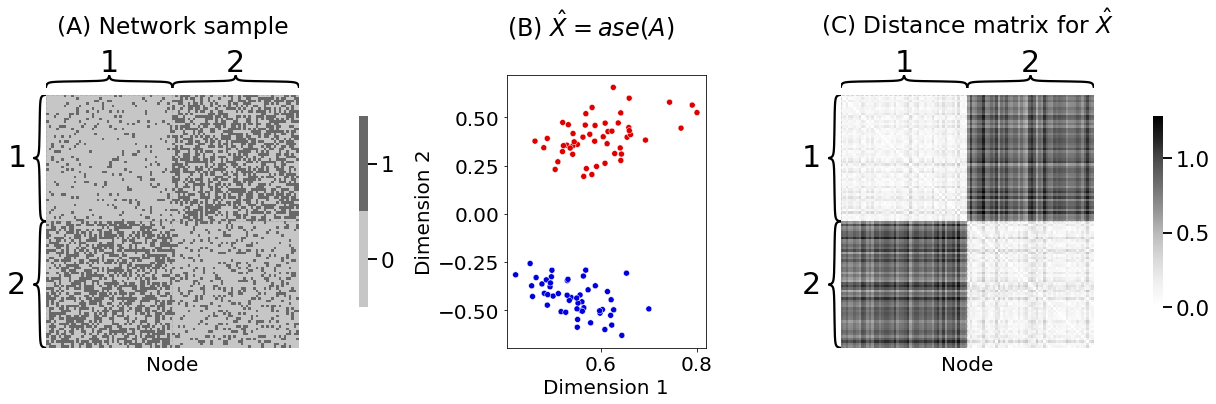
\includegraphics[width=\linewidth]{representations/ch6/Images/diss.png}
    \caption[ASE with indefinite probability matrix]{\textbf{(A)} a sample of a random network with an indefinite block matrix, and hence, and indefinite probability matrix, \textbf{(B)} a scatter plot of the estimated latent positions via \texttt{ase}, \textbf{(C)} the distance matrix between pairs of estimated latent positions.}
    \label{fig:ch6:dimest:diss}
\end{figure}

We visualize the sample of the random network with a non positive semi-definite probability matrix in Figure \ref{fig:ch6:dimest:diss}(A), where it is fairly evident that between-community connections (the off-diagonal blocks of the adjacency matrix in the upper-right and lower-left corners) are more frequent than within-community connections (the on-diagonal blocks of the adjacency matrix). This intuitively reflects the idea that the underlying random network has a non positive semi-definite probability matrix. The estimated latent positions are shown in Figure \ref{fig:ch6:dimest:diss}(B). Notice that even though the block matrix (and consequently the probability matrix) of the underlying random network is not positive semi-definite, that \texttt{ase} still produced a meaningful embedding, in that nodes from the same community were still more similar than nodes from different communities. This insight can be confirmed by looking at the pairwise distance matrix, in Figure \ref{fig:ch6:dimest:diss}(C). While some of the strategies discussed, such as the \texttt{omni} embedding \cite{Levin2017}, were developed prior to these results, it is likely that they produce principled estimates of latent positions even under non positive semi-definite structures, as our experiments in Figure \ref{fig:ch6:multinet:omni:pests}(B) showed, where we used \texttt{omni} to recover the non positive semi-definite structure of the alien probability matrix.

Hopefully, this provides a level of credence to the idea that spectral embeddings are extremely flexible, and can be used to derive latent structure from network samples across many (not just positive semi-definite) contexts.

\newpage
